\documentclass{sig-alternate}
\usepackage[numbers, sort, compress]{natbib}
\usepackage{graphics}
\usepackage{graphicx}
\usepackage{epstopdf}
\usepackage{color}
\usepackage{hyperref}
\usepackage{pdfsync}
\usepackage{mdwlist}
\usepackage{booktabs}


\begin{document}

\conferenceinfo{XSEDE '12, July 16-20, 2012, Chicago, USA.} {}
\CopyrightYear{2012}
\crdata{}
%\clubpenalty=10000
%\widowpenalty = 10000

% \title{BigJob: Lessons of Supporting High Throughput High Performance
%   Ensembles on XSEDE}

%\title{The Anatomy of a successful ECSS Project: Leveraging Expertise
%  of Users, Software-providers and XSEDE Personnel}

\title{The Anatomy of Successful ECSS Projects: Lessons of Supporting
  High-Throughput High-Performance Ensembles on XSEDE}

\numberofauthors{6}
\author{
\alignauthor Melissa Romanus\\
       \affaddr{CAC/ECE}\\
	\affaddr{Rutgers University} \\
       \affaddr{94 Brett Road} \\
	\affaddr{Piscataway, NJ} \\
       \email{melissa@cac.rutgers.edu}
\alignauthor Pradeep Kumar Mantha\\
       \affaddr{Center for Computation and Technology}\\
       \affaddr{Louisiana State University}\\
       \affaddr{216 Johnston}\\
       \affaddr{Baton Rouge, LA}
       \email{pmanth2@cct.lsu.edu}
\and
\alignauthor Matt McKenzie\\
       \affaddr{National Institute for Computational Sciences}\\
       \affaddr{Oak Ridge, TN} \\
       \email{mmckenz9@utk.edu}
\alignauthor Tom Bishop\\
       \affaddr{Louisiana Tech University}\\
       \affaddr{Ruston, LA} \\
       \email{bishop@latech.edu }
\alignauthor Emilio Gallichio\\
       \affaddr{ BioMaPS Institute - Rutgers University}\\
       \affaddr{Piscataway, N} \\
       \email{emilio@biomaps.rutgers.edu }
\and
\alignauthor Andre Merzky\\
       \affaddr{Center for Computation and Technology}\\
       \affaddr{Louisiana State University}\\
       \affaddr{216 Johnston}\\
       \affaddr{Baton Rouge, LA}\\
       \email{andre@merzky.net}
\and       
\alignauthor Yaakoub El Khamra\\
       \affaddr{Texas Advanced Computing Center}\\
       \affaddr{The University of Texas at Austin} \\
       \affaddr{Austin TX} \\
       \email{yaakoub@tacc.utexas.edu}       
\alignauthor Shantenu Jha\\
     \affaddr{The Cloud and Autonomic Computing Center}\\
     \affaddr{Rutgers University}\\
      \affaddr{94 Brett Road}\\
      \affaddr{Piscataway, NJ}
     \email{shantenu.jha@rutgers.edu}
}

\maketitle


\begin{abstract}
The Extended Collaborative Support Service (ECSS) of XSEDE is a means
of providing support for advance user requirements that cannot and
should not be supported via a regular ticketing system. Recently two
ECSS projects were awarded by XSEDE management to support the
high-throughput of high-performance (HTHP) molecular dynamics (MD)
simulations; both of these ECSS projects are using SAGA-based
Pilot-Jobs approach as the technology required to support the HTHP
scenarios.  More significantly, these projects were envisioned as
three-way collaborations: between the application stake-holders,
advanced/research software development team and the resource
providers. In this paper, we describe the aims and objective of these
ECSS projects, how the deliverables have been met, and some
preliminary results obtained. We also describe how SAGA has been
deployed on XSEDE as a precursor to the seamless uptake of BigJobs.
\end{abstract}


\newif\ifdraft \drafttrue \ifdraft
\newcommand{\mrnote}[1]{{\textcolor{green} { ***MR: #1 }}}
\newcommand{\jhanote}[1]{ {\textcolor{red} { ***SJ: #1 }}}
\newcommand{\yyenote}[1]{ {\textcolor{cyan} { ***YYE: #1 }}}
\newcommand{\pmnote}[1]{ {\textcolor{blue} { ***PM: #1 }}}
\newcommand{\todo}[1]{ {\textcolor{red} { ***TODO: #1 }}}
\newcommand{\fix}[1]{ {\textcolor{red} { ***FIX: #1 }}}
\newcommand{\reviewer}[1]{} \else \newcommand{\yyenote}[1]{}
\newcommand{\mrmnote}[1]{} \newcommand{\pmnote}[1]{}
\newcommand{\jhanote}[1]{} \newcommand{\todo}[1]{ {\textcolor{red} {
      ***TODO: #1 }}} \newcommand{\fix}[1]{} \fi



\category{D.1.3}{Software}{Concurrent Programming}{ Distributed programming/parallel programming} 
\category{J.3}{Computer Applications}{Bioinformatics}

\section*{General Terms}{Design,Measurement,Theory}

 \keywords{}

\section{Introduction}
\yyenote{SJ can you have a look at this and massage it to your liking?}

The Extended Collaborative Support Service (ECSS) pairs members of the XSEDE
user community with expert staff for an extended period to work together to
solve challenging science and engineering problems through the application of
cyberinfrastructure~(\cite{ECSS_webpage}). In depth staff support, lasting a few
weeks to up to a year in length, can be requested at any time through the XSEDE
allocations process. Expertise is available in a wide range of areas, from
performance analysis and petascale optimization to the development of community
gateways and work and data flow systems.

In this paper we discuss two ECSS projects that overlap in both scientific
endeavor and computational challenges. The success of these two projects is
attributed to the strong interaction and familiarity between ECSS staff and
infrastructure developers. The collaboration between system administrators and
middleware developers lead to the deployment of production-grade infrastructure
that is currently being used by the scientists.

The computational challenges are circumvented through innovative solutions in
distributed and high throughput computing thus satisfying the computational
scientists' requirements. The development and deployment of these tools is left
to computer scientists, developers and programmers of infrastructure and
middleware. The ECSS staff supports both scientists and tool developers in both
deployment, bug reporting, testing, fixes and system issues. This three-way
split insulates the scientists from the ``plumbing'' and the ECSS consultants
from middleware development. The successful distribution of labor translates
to reduced effort across the board, higher scientific output and less issues.
Furthermore, the fact that middleware developers are in constant communication
with ECSS consultants improves the middleware itself. The ECSS consultants
report to the developers issues ranging from middleware misbehavior,
choke points, scaling issues, un-necessary increases in file system load and so
on. The developers resolve these issues, test and re-deploy while maintaining
backwards compatibility, leaving the scientists unaffected.

The overlap of two ECSS projects with the same computational challenges lead to
increased efficiency. The same tools, infrastructure and documentation prepared
for one ECSS project is being used by another, similar project. There was,
however, a slight increase in the number of issues reported: twice the number
of users meant more bugs reported. This is only expected, and to some extent
quite welcome. At the end of the day, however, two ECSS projects are nearing
completion ahead of schedule for the cost of just one project.

In this paper we discuss the ECSS projects, the computational challenges
involved and the middleware solution. We also discuss in detail the lessons
learned from testing and deploying on different machines and collaborating
across the three disciplines of scientists, middleware developers and ECSS
consultants.



\section{Scientific Background and Motivation}

Overlapping two ECSS projects that face the same computational challenges
with the same ECSS consultant and middleware developer team is an efficient
use of XSEDE resources. What follows is scientific background of both ECSS projects
and the common computational challenges.

\subsection{Distributed and Loosely Coupled Parallel Molecular Simulations
Using the SAGA API}
The first ECSS project~(\cite{RonLevy}) is part of an intense effort to
understand
important aspects of the physics of protein-ligand recognition by
multidimensional replica exchange (RE) computer simulations. These are
compute intensive calculations which require large numbers (103-104) of
loosely coupled replicas and long simulation times (days to weeks). In
conventional implementations of RE, simulations progress in unison and
exchanges occur in a synchronous manner whereby all replicas must
reach a pre-determined state (typically the completion of a certain
number of MD steps), before exchanges are performed. This synchronous
approach has several severe limitations in terms of scalability and
control. First of all, Sufficient dedicated computational resources must
be secured for all of the replicas before the simulation can begin
execution. Second, the computational resources must be statically
maintained until the simulation is completed. Third, failure of any
replica simulation typically causes the whole calculation to abort.


\subsection{High Throughput, High Performance MD Studies of the Nucleosome
using SAGA-based Pilot-Jobs}
The second ECSS project focuses on high throughput, high performance molecular
dynamics studies of the nucleosome~(\cite{TomBishop}). Genomes in higher
organisms
exist for most of the cell's cycle as a protein-DNA complex called chromatin.
Nucleosomes are the building blocks of chromatin, thus, nucleosome stability and
their positioning within chromatin impacts virtually all genetic processes
including: transcription, replication, regulation, repair.

The primary goal of the proposed simulation studies in this project is to
investigate by means of all atom molecular dynamics simulations variations in
nucleosome structure and dynamics arising from DNA chemical modifications and
from receptor binding. This is being accomplished by means of a hierarchical
modeling and simulation strategy that utilizes high throughput, high
performance all atom molecular dynamics simulation techniques. The project is
on track to generate approximately 140,000ns of molecular dynamics simulation
data for at least 150 different realizations of the nucleosome.


\subsection{Computational Challenges}

Most run-time environments and tools for high-performance and
distributed computing assume either that there is a single instance of
a task/simulation that must be executed, or there is a complex
dependency (and thus workflow) associated with distinct ``tasks''.
However, in an increasingly large number of scientific problems, there
is a need for a large number of similar tasks to be run concurrently.

There is a fundamental need for supporting ensemble-based simulations
(ES) across a range of disciplines, including but not limited to
biological, chemical, environmental and material sciences; existing
capabilities are insufficient to support ES at scale. 

Depending upon the specific problem, the identical tasks may vary in
the number of cores required, or in the degree of coupling between the
tasks.  Either way there are missing capabilities to support the
multiple similar tasks that need to run concurrently


% In other words, an ideal framework would be interoperable with a range
% of modeling software and extensible to emerging computational
% platforms such as clouds and GPU-computers, and thus usable on a range
% of underlying distributed resources and independent of the
% machine/resource-specific middleware and services.


The challenge for ES is that of managing multiple tasks concurrently;
typically for a given science problem this number does not vary during
the lifetime of the execution. Although, similar to workflows, the
objective is the reduction of the makespan~\yyenote{What the hell does
makespan mean}, but in contrast to
traditional workflows, there isn't a multi-level dependency to solve
and thus the execution of ES is not fundamentally a challenging
scheduling problem.

The concurrent support of multiple similar simulations requires the
efficient and transparent management of a large number of ensembles,
possibly on many heterogeneous resources. The same run-time solution
should be applicable to a range of physical model sizes -- from
thousands of atoms to hundreds of thousands of atoms.%  Effectively
% manage large-scale data transfers and analysis, and all of
The above should be addressed without being tied to a specific
underlying application kernel or physical infrastructure. 
 
Although multi-site resources have the potential for substantial
improvements in time-to-completion of ES, the capability to
effectively utilize NSF's National Production Cyberinfrastructure
XSEDE is missing, as developing, deploying and executing these
capabilities to use the collective power of XSEDE is a challenging
undertaking, which cannot be carried forth by a single group or
sustained without the involvement of all stakeholders: scientists,
resource providers and software-developers.

\section{ECSS Projects}

We found ourselves with two ECSS projects aligned in infrastructure, tools and
workflow. This effort was the proverbial: ``two for the price of one'' sort
of undertaking. The deployment of the infrastructure (SAGA and BigJob), the
development of workflows and data management tools are all requirements
for both ECSS projects. In what follows we outline level of effort involved
in both projects.

% \subsection{Formal description of What is ECSS - from mgmt perspective}
% 
% \subsection{Why ECSS for this requirement?}
% 
% \jhanote{(i) from a users perspective? (ii) from a software
%   providers/developers perspective? (iii) from a resource providers
%   perspective?}
% 
% \subsubsection{Users} (i) single point of contact, (ii) integrated capabilities,
% (iii) capabilities not bound to a specific resource; scalable across
% different resources
% 
% \subsubsection{Software Providers} Point (iii) above, but also focused support
%and
% consultant on individual machines.
% 
% \subsubsection{From XSEDE-RP} (i) Gain more than system level support/expertise, (ii)
% common/shared knowledge and thus spread across community, (iii)
% derived from previous point, if successful, at the end of ECSS
% XSEDE/RP have a new capability/ability to provide an advanced service

\subsection{Effort Involved: Distributed and Loosely Coupled Parallel Molecular Simulations
Using the SAGA API}

The reliance on a static pool of computational resources and no
fault tolerance prevents the synchronous RE approach from being a
solution on XSEDE resources. We therefore implemented asynchronous
parallel replica exchange conformational sampling algorithms together
using the SAGA distributed computing framework to enable dynamic
scheduling of resources and adaptive control of replica
parameters. The basic idea is to allow pairs of replicas to contact
each other to initiate and perform exchanges independently from the
other replicas. Because replicas do not rely on centralized
synchronization steps, asynchronous exchange algorithms are scalable to an
arbitrary number of processors. These algorithms also circumvent
the need to maintain a static pool of processors and therefore
can be distributed logically and physically across XSEDE resources.
In that case, the number of concurrent replicas changes dynamically
depending on available resources. This mode of execution is particularly
suitable for implementation within using SAGA and tools-based upon SAGA.

In terms of scope, assistance from XSEDE personnel was needed to: (i) set up and
harden the necessary SAGA, BigJob and Advert Service software infrastructures on
Ranger, Lonestar, Kraken, and Nautilus and deploy the scientific software
IMPACT~(\cite{IMPACT}) and AMBER~(\cite{AMBER}) (ii) work with the
users to enable launching NAMD, IMPACT, and AMBER distributed jobs using the
SAGA BigJob framework, (iii) work with users to develop customized RE scripts
and with the SAGA team to test and validate relevant adaptors aimed at
conducting synchronous and asynchronous file-based replica exchange simulations
in the context of the SAGA-based Pilot-Job framework, and (iv)  document and
validate the usage of the Replica-Exchange framework on XSEDE.

Hardening the software infrastructures requires profiling and benchmarking the
workflow management tools (SAGA, BigJob) to measure overhead and identify any
load spikes on the filesystems. Once the bottlenecks and problem areas were
identified, they were resolved by the SAGA development team with help from
the ECSS consultants. The SAGA development team handled all major feature
implementations and bug fixes required for this effort including custom
adaptors for Lonestar and Ranger. 

\subsection{Second ECSS Project: High Throughput, High Performance MD Studies of the Nucleosome
using SAGA-based Pilot-Jobs}
The second ECSS project focuses on high throughput, high performance molecular
dynamics studies of the nucleosome~(\cite{TomBishop}). Genomes in higher
organisms
exist for most of the cell's cycle as a protein-DNA complex called chromatin.
Nucleosomes are the building blocks of chromatin, thus, nucleosome stability and
their positioning within chromatin impacts virtually all genetic processes
including: transcription, replication, regulation, repair.

The primary goal of the proposed simulation studies in this project is to
investigate by means of all atom molecular dynamics simulations variations in
nucleosome structure and dynamics arising from DNA chemical modifications and
from receptor binding. This is being accomplished by means of a hierarchical
modeling and simulation strategy that utilizes high throughput, high
performance all atom molecular dynamics simulation techniques. The project is
on track to generate approximately 140,000ns of molecular dynamics simulation
data for at least 150 different realizations of the nucleosome.

This project's work flow requires simulating as many as 85 independent systems
simultaneously. For each system, every nanosecond of simulation is an HPC event
that requires approximately 50 MB of input, generates 4 GB of output and scales
efficiently from as few as 32 to as many as 512 cores. On 64 processors the run
time for a single 1 ns simulation task is approximately 6 hrs. The goal is to
accumulate 50 ns of simulation for the entire set of 85 systems (4,250 1 ns
simulation tasks in total) as quickly as possible, then select a subset of
systems from the ensemble for which 500 ns of additional dynamics will be
accumulated. If we chose only 10 systems for continued studies this is still
5,000 1ns simulation tasks to be completed. To reduce the time-to-completion of
the entire workload and to manage simulation inputs/outputs on scratch file
systems, we are intend to use multiple XSEDE resources simultaneously and
therefore require data staging.

The major differences in usage modes between the two ECSS projects is that this
project requires: (i) a much larger number of ensembles running concurrently and
for longer durations, (ii) the chaining of ensembles, (iii) much larger
data-volumes, (iv)  BigJob infrastructure that currently does not support the
co-movement and coordinated movement of data(files) in conjunction with ensemble
placement. Bigjob file movement capabilities are being enhanced to provide
such support.

Support from ECSS consultants is necessary for this ECSS, specifically for disk
and storage bottlenecks. Data management is a growing issue, especially with
varying transfer rates, less-than-portable transfer mechanisms and so on.

\subsection{Common Effort across Both Projects}

Both projects share the same basic infrastructure in terms of software and
hardware. Both projects share consultant teams, software developers and some of
the scientific tools. The workflows are not dissimilar either: both ECSS
projects intend to launch pilot jobs in a dynamic workflow on distributed
resources, stage and collect data and so on.

With a view towards making these capabilities more publicly accessible and
widely used, The ECSS project also included developing a prototype
Replica-Exchange Gateway. This gateway was developed using the
DARE~(\cite{DARE})
scientific gateway framework. This scientific gateway prototype is hosted
on IU's Data Quarry machine~(\cite{DataQuarry}). Furthermore, all tools,
utilities, and components will be placed in CSA space on Ranger,
Lonestar, and Kraken. All code and corresponding documentation will also be
maintained in a local revision control software repository which is publicly
available.


\section{Methodical Solution and Technology}


\subsection{SAGA: Standards-based Access to the Resources Layer}

The Simple API for Grid Applications (SAGA)~(\cite{saga_url}) is an
implementation of an Open Grid Forum (OGF) Technical Specification
that provides a common and consistent high-level API for the most
commonly required functionality to construct distributed applications.
It also provides a high-level API to construct tools and frameworks to
support distributed applications. The functional areas that are
supported by SAGA include job-submission, file transfer and access, as
well as support for data streaming and distributed coordination. SAGA
provides both a syntactic and semantic unification via a single
interface to access multiple, semantically distinct middleware
distributions.

%SAGA is an API that provides the basic functionality for developing
%distributed applications, tools and frameworks. 

The key advantages of the development using SAGA include, but are not
limited to: i) to provide a general-purpose, commonly used yet
standardized functionality, while hiding complexity of heterogeneity
of back-end resources, ii) to provide building blocks for constructing
higher-level functionality and abstractions, iii) to provide the means
for developing broad range of distributed applications such as
gateways, workflows, application management systems, and runtime
environments. Interestingly, SAGA provides an integrated, light-weight
approach to support scripting for building distributed applications.

Different aspects of SAGA appeal to different groups. The
standardization of SAGA as an OGF Standard is important because it
makes it more likely that production infrastructures, like NSF XSEDE,
EU PRACE and Open Science Grid, will support SAGA. Having SAGA
deployed and tested on these systems makes it readily available for
users and developers of national Cyberinfrastructure projects. The
fact that SAGA is an OGF technical specification also makes SAGA
highly appealing to application frameworks, services and tool
developers, which is quite understandable, as it not only simplifies
their development but also makes for scalable, extensible and
sustainable development. Users find the simple and extensible
interface providing the basic abstractions required for distributed
computing is very appealing to add their own ``functionality'' to a
core base of functionality. Furthermore, SAGA is now part of the
``official'' access layer for the \$121M NSF TG/XSEDE
project~(\cite{xsede_url}), as well as for the world largest distributed
infrastructure EGI~(\cite{egi_url}).

The SAGA API provides the base abstractions upon which tools and
frameworks that provide higher-level functionality can be
implemented. Ref.~(\cite{saga_url}) discusses distributed application
frameworks and run-time systems that SAGA has been used to develop
successfully. 

\begin{figure}[t]
\centering
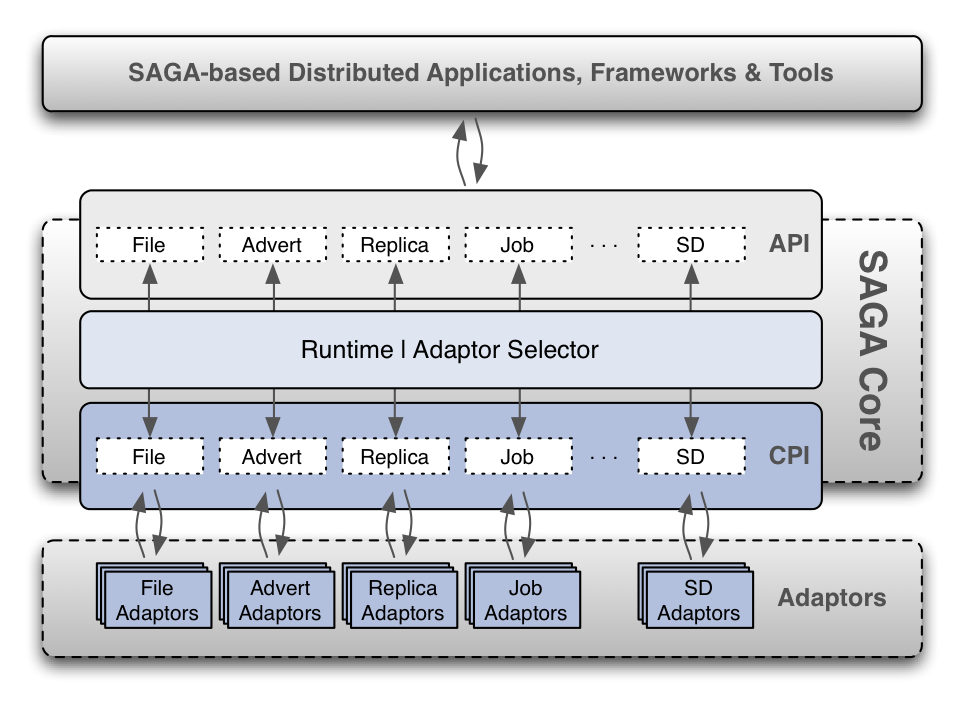
\includegraphics[width=0.44\textwidth]{./figs/saga-architecture-1}
\caption{\textbf{SAGA Overview: } SAGA is an OGF technical
  specification that provides a common interface to heterogeneous DCI
  -- hitherto typically Grid systems.  The implementation of the
  SAGA~(\cite{saga_url}) specification consists of a high-level {\it
    API}, the SAGA {\it Engine} providing that API, and backend,
  system-specific {\it Adaptors}.  The engine is a lightweight,
  highly-configurable dynamic library that manages call dispatching
  and the dynamic runtime loading of the middleware adaptors.  Each of
  these adaptors implements the functionality of a specific functional
  package (e.g., job adaptors, file adaptors) for a specific
  middleware system. Adaptors are also realized as dynamic libraries.}
 \label{fig:saga-overview}
\end{figure}

A SAGA implementation consists of a high-level API, the SAGA
Engine providing that API, and backend, middleware/systems specific
adaptors. Each of these adaptors implements the functionality of
a functional package (e.g., job adaptors, file adaptors) for a
specific middleware system. The engine is a dynamic library that
manages call dispatching and the runtime loading of the middleware
adaptors. Adaptors are also realized as dynamic libraries. The SAGA
API has been used (in C++, Python and Java versions) to provide almost
complete coverage over nearly all grid and distributed computing
middleware/systems, including but not limited to Condor, Genesis,
Globus, UNICORE, LSF/PBS/Torque and Amazon EC2.

SAGA is currently used on production Cyberinfrastructure in several
ways. Admittedly the number of first-principle distributed
applications developed is currently low, but SAGA has been used to develop
``glue-code'' and tools that are used to submit and marshal jobs and
data across and between heterogeneous resources. Specifically, it has
been used to support multiple computational biology applications that
use high-performance and high-throughput molecular dynamics (MD)
simulations.

SAGA has been used to develop a standards-based library for Science
Gateways to easily utilize different distributed resources; some
science domains that are using SAGA-based Science Gateways include
gateways to support next-generation sequencing, docking and
high-throughput of ensembles.

HPDC infrastructure is by definition comprised of a set of resources
that is fluctuating -- growing, shrinking, changing in load and
capability. This is in contrast to a static resource utilization model
traditionally a characteristic of parallel and cluster computing. The
ability to utilize a dynamic resource pool is thus an important
attribute of any application that needs to utilize HPDC infrastructure
efficiently. Applications that support dynamic execution have the
ability to respond to a fluctuating resource pool, i.\,e., the set of
resources utilized at time (T), $T=0$ is not the same as $T>0$.  Thus,
the need to support dynamic execution is widespread for computational
science applications; here we accomplish this by using the SAGA-based
Pilot-Job.

\subsection{SAGA-based Pilot-Job: BigJob}

\yyenote{So first off, this pilot-job definition does not explain why we chose
to use pilot jobs to overcome the computational challenges. Furthermore, the
use of the word speed in relation to calculations means FLOPS, this is wrong.
The use of the word ALLOCATION is also wrong. In XSEDE, allocation means one and
only one thing and this is NOT it. We need a clear, layman's definition of what
pilot jobs are in relation to the computational  challenge. The following is
NOT.}
Workload management and resource scheduling can lead to significant dynamic 
fluctuations in workloads and resources, reducing the overall efficiency
and speed of the desired calculations. 
A common approach for decoupling  
these competing allocation problems is the use of \emph{pilot-jobs (PJ)}. 
\mrnote{This is the point where we should first try to define a pilot job 
in a clear manner} The  PJ
abstraction is also a promising route to address additional requirements of
distributed scientific applications~(\cite{ko-efficient,bigjob_cloudcom10}),
such
 as application-level scheduling.

A SAGA-based PilotJob, BigJob (BJ)~(\cite{bigjob_web,saga_bigjob_condor_cloud}),
is a general-purpose pilot-job framework. BigJob has been used to support
various execution patterns and execution
workflows~(\cite{async_repex11,repex_ptrsa}). For example, SAGA-BigJob was used
to execute scientific applications categorized as embarrassingly parallel
applications and loosely coupled applications on scalable distributed
resources~(\cite{ecmls_ccpe10, dare-ecmls11})

Figure~\ref{fig:figures_re_bigjob_interactions} illustrates the
architecture of BJ. BJ utilizes a Master-Worker coordination
model. The BigJob-Manager is responsible for the orchestration of
pilots, for the binding of sub-tasks. For submission of the pilots,
SAGA relies on the SAGA Job API, and thus can be used in conjunction
with different SAGA adaptors, e.\,g.\ the Globus, the PBS, the Condor
and the Amazon Web Service adaptor. Each pilot initializes a so called
BJ-agent. The agent is responsible for gathering local information and
for executing tasks on its local resource. The SAGA Advert Service API
is used for communication between manager and agent. The Advert
Service (AS) exposes a shared data space that can be accessed by
manager and agent, which use the AS to realize a push/pull
communication pattern.  The manager pushes a sub-job to the AS while
the agents periodically pull for new sub-jobs. Results and state
updates are similarly pushed back from the agent to the
manager. Furthermore, BJ provides a pluggable communication \&
coordination layer and also supports alternative c\&c systems,
e.\,g.\ Redis~(\cite{redis}) and ZeroMQ~(\cite{zmq}).

In many scenarios it is beneficial to utilize multiple resources,
e.\,g.\ to accelerate the time-to-completion or to provide resilience
to resource failures and/or unexpected delays.  BJ supports a wide
range of application types, and is usable over a broad range of
infrastructures, i.\,e.\ it is general-purpose and extensible
(Figure~\ref{fig:figures_re_bigjob_interactions}). In addition there
are specific BJ flavors for cloud resources such as Amazon EC2 and
Microsoft Azure that are capable of managing set of VMs, as well as a
BJ with a Condor-G based backend.

\yyenote{We go to incredible lengths to discuss what this is in complicated
terms but do not say what this means to an end user, how this relates to the
scientific problem. We either tie this in or remove for lack of cohesion. }
BJ supports dynamic resource additions/removals as well as late
binding. The support of this feature depends on the backend used. To
support this feature on top of various BigJob implementations that are
by default restricted to single resource use (e.\,g.\ BJ), the concept
of a BigJob pool is introduced. A BigJob pool consists of multiple BJs
(each BigJob managing one particular resource). An extensible
scheduler is used for dispatching WUs to one of the BJs of the pool
(late binding). By default a FIFO scheduler is provided.

\begin{figure}[t]
  \centering
  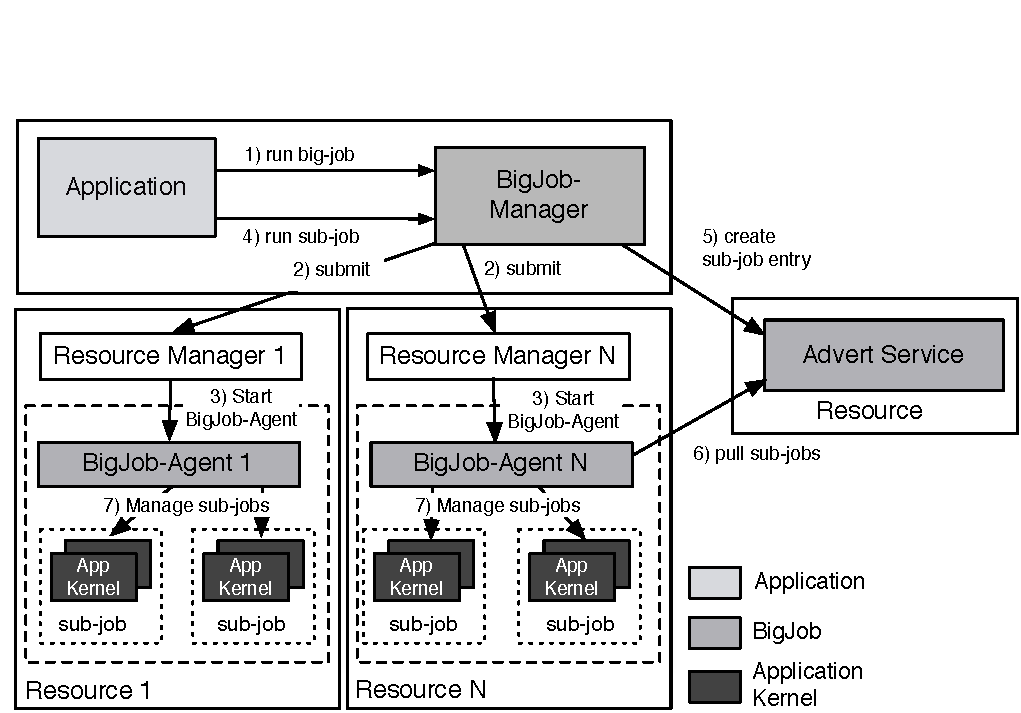
\includegraphics[width=0.40\textwidth]{./figs/re_bigjob_interactions}
   \caption{\textbf{BigJob Architecture:} The core of the framework,
     the BigJob-Manager orchestrates a set of pilots. Pilots are
     started using the SAGA Job API. The application submits WUs, the
     so-called sub-jobs via the BigJob-Manager. Communication between
     the BJ-Manager and BJ-Agent is done via a shared data space, the
     Advert Service. The BJ-Agent is responsible for managing and
     monitoring sub-jobs. From Ref.~(\cite{saga_bigjob_condor_cloud})}
        \label{fig:figures_re_bigjob_interactions}
\end{figure}



\section{SAGA and BigJob on XSEDE}
This section describes the deployment, testing, and documentation of
SAGA and BigJob on XSEDE resources.


\subsection{SAGA: Simple API for Grid Applications}
 \label{ssec:saga}
 
\yyenote{Why are we repeating the definition of saga and its architecture here?
We had an entire subsection about saga. SJ we either remove this or fix it so
that it only includes xsede related aspects of SAGA, nothing about SAGA's
details.}
 
XSEDE is inherently a very complex infrastructure.  Given the wide
range of user groups and application use cases it aims to address,
and the large number and the diversity of participating resource
providers, this is to be expected.  Complex systems are though
usually very difficult to use, as that complexity and the underlying
resource diversity often translates into complicated user tools and
interfaces.  The relatively clean architecture of XSEDE is, to some
extent, addressing this problem, but is, in itself and at this point
in time, a moving target.

The Simple API for Grid Applications (SAGA) aims to address a part of
that problem, by providing a well defined and stable API, which
exposes those operations which are required on application level, but
encapsulates the complexity of translating them into the respective
operations on the XSEDE infrastructure.  In other words: SAGA tries
to move the complexity of dealing with distributed
cyberinfrastructures like XSEDE out of the application, and into the
SAGA implementation layer, while providing the semantics necessary to
efficiently implement distributed applications which can utilize
XSEDE.

A SAGA implementation is comprised of a
core API, which defines the overall API structure, and a set of API
packages, covering topics like job submission and management, file
access and movement, and the coordination of distributed application
components.  Multiple implementations of SAGA exist, most notably a
C++/Python implementation, which is deployed on all major XSEDE
clusters (see sec.~\ref{ssec:csa}).  A newly emerging pure python
implementation (Bliss) is expected to replace it later in 2012 --
Bliss' development and testing is specifically targeting XSEDE and
FutureGrid as target platforms.

\subsection{CSA Deployment on XSEDE Machines}
 \label{ssec:csa}
 
SAGA and BigJob are deployed on all major XSEDE
machines~(Table \ref{table:CSA-Deployments}) (ranger,
kraken, lonestar, trestles, blacklight, steele) as well as FutureGrid machines
(india, sierra, hotel, alamo). While it is possible to install and
use SAGA and BigJob each user's directory, it would not be without a non-trivial
amount of effort in configuration and maintenance. Furthermore, having a
central location on each machine where SAGA is deployed as a community code
saves ECSS consultants time and effort in maintaining the installation and
supporting its users. XSEDE continues the TeraGrid model of providing Community
Software Areas (CSA) to communities, which basically is a system
level area where software packages can be shared among a community of users.
Therefore it was only logical to deploy SAGA and BigJob in a CSA space on XSEDE
and FutureGrid machines.

The installation and update are semi-automatic: a set of deployment
scripts are used to manually trigger the update. The update can encompass an
individual machine or all machines, an individual SAGA component or the entire
SAGA/BigJob installation. The set of supported components includes the SAGA core
libraries, different API packages, the supported
middleware adaptors for each machine, the python bindings, and the
BigJob package and its dependencies. Each installation automatically creates a
README file that describes the installed components, and documents settings
required to use the installation, settings such as the
\texttt{LD\_LIBRARY\_PATH} and so on. A module file is also generated and on
some hosts is symbolically linked to the system default module path. 

After each update, a set of unit tests is run \textit{on the
target machines} to ensure that not only the updated version is deployed, but
more importantly, that it is correctly installed and
configured for that target machine. The unit tests range from basic
(low-level) environment testing, to application level test runs of a
BigJob application. The test README, module file and test results
are all committed to the central SAGA code repository, and
(partially) used to document the current state of deployment on the
SAGA deployment wiki.

\begin{table}
\begin{center}
\begin{tabular}{ll}
\toprule
\textbf{Machine}  & 
\textbf{Adaptors Supported} 
\\ \midrule
Kraken   & 
X509, Globus, SSH, Torque/PBS
\\ \midrule
Ranger   & 
X509, SSH
\\ \midrule
Lonestar & 
X509, Globus, SSH
\\ \midrule
Blacklight & 
X509, Globus, SSH, Torque/PBS
\\ \midrule
Steele & 
X509, Globus, SSH, Torque/PBS
\\ \midrule
Trestles & 
X509, Globus, SSH, Torque/PBS
\\ \bottomrule
\end{tabular}
\caption{CSA Deployments on XSEDE Resources}
\label{table:CSA-Deployments}
\end{center}
\end{table}

\subsection{Developments and Setbacks}

The use of multiple resources brings about certain challenges which tend to reappear in 
every distributed ECSS project. For example, each of the machines (Lonestar, Ranger, 
Kraken, and Trestles) may have different user environments, different shells, and 
different invocation order of startup profiles on both login and compute nodes. A major 
complication is the differences in system versions of Python. Most machines have an older 
version of Python supplemented by a Python module. The Python module did not typically 
include the tools required to easily install user-side python modules. Therefore, a fresh 
installation of Python is always present in the shared CSA space. A similar issue is 
encountered with GCC compiler versions as well.

A slightly more intricate issue is the use of custom ``mpirun'' wrappers. On
Ranger/Lonestar, it is ``ibrun'', on Kraken, it is ``aprun''. These wrappers
massage the nodelist files, aggregate important environment variables to launch
with the application and so on. Modifications have to be made the launch
mechanism in BigJob to account for the use of these scripts.

Job submission is another interesting issue. Lonestar and Ranger use SGE, while
Kraken and Trestles use PBS. While SAGA retains the ability to submit jobs
through the Globus (\cite{Globus}) job adaptor, it is an unnecessary burden on
users. Furthermore, when Globus submitted jobs fail, they generate a very
lengthy error report without much useful information. Both projects needed an
immediate, clear, and fail safe mechanism to submit jobs and this lead to the
development of the \textit{pbs-ssh} and \textit{sge-ssh} plugins to support both
PBS and SGE. The plugins enable local/remote launch of BigJob agents using
traditional PBS/SGE script over SAGA ssh job adaptors.

The last issue is a user-side issue. The more diverse the machines and their
environments are, the more diverse the documentation and the higher the entry
barrier. For example, Kraken requires the initialization of a ``myproxy'' for
successful job submission, whereas Ranger and Lonestar do not. These small  but
critical differences can mean the difference between successful several thousand
core jobs or a week of waiting in the queue to exit on an error.


\subsection{Testing and Documentation Process}

The source code for SAGA and BigJob is stored in a
git repository (\cite{bigjob_web}). A github wiki is used to store user guides
for each of the individual XSEDE machines. The BigJob wiki stores all
information about the installation and configuration of BigJob. Only users of
the BigJob development group can edit this wiki. This wiki is public and can be
shared amongst all collaborators. Public wikis also serve as a way to promote
other people to use and try BigJob for their scientific needs.

A BigJob CSA release is the result of a production pipeline. Any newly developed
features, code modifications and bug fixes are created in branches. After
review, branches are merged onto the master branch of the git repository. The
main developer determines when a new version of BigJob will be released. 

Members of the BigJob development team then checkout the release candidate
version from git and test on XSEDE resources. Tests include checking output and error logs, 
ensuring that the installation is seamless, ensuring backwards compatibility with existing 
scripts and workflows, monitoring the submission environment and so on. This rigorous quality 
assurance process is repeated for every machine.

For every machine there are least two machine-specific examples in the git
repository and CSA space. These are example BigJob scripts that run a job in
both single and multiple communication (i.e. MPI) mode. The first script simply
runs a shell ``/bin/date'' command. Since the ECSS project supports molecular
dynamics simulations, the second script runs a real AMBER MD simulation. These
scripts test the basic functionality of BigJob using the CSA installations and
serve as standard tests.

With each testing phase, the testing team follows the instructions in the user
guide, step-by-step, in a sterile user environment to make sure the
documentation is correct and the updates are backwards compatible.
Naturally, each machine has scripts that are tailored to the batch queue submission
system on that machine -- i.e. Ranger uses an SGE submission while Kraken uses
PBS. By testing these across multiple job submission systems, we are also
exercising the backend job submission BigJob code to make sure that changes have
not negatively affected the submission. After the jobs finish successfully, the
output is analyzed to validate the results. The AMBER scripts also serve as a
test for the AMBER installations on the appropriate machines, and allow the
testing team to check that AMBER starts and runs normally.

After testing is complete, the python code is pushed to the Python Package Index
(\textit{pypi}). This code is then deployed into the CSA space using pypi.
Careful consideration is taken to ensure that the updates to CSA space
will not impact any current users of BigJob on the XSEDE resources. Another round of testing 
is then completed to verify that the CSA installations are working and no changes to 
the users' environments are required. Any corresponding documentation on the 
github wiki is updated to reflect the changes.

In addition to this release process, the BigJob team is engaged with members
of the ECSS team in order to resolve any system-level issues that may arise.
These issues may include but are not limited to differences in schedulers or MPI
implementations. Additionally, the scientific collaborators use the wiki as a
starting point to run their applications on XSEDE machines. The scripts and
associated documentation explain how to use BigJob with their own applications
simply by specifying the job description. 

If the end users encounter any issues, the BigJob team works with the ECSS
consultants to resolve the problems. A mailing list including ECSS consultants,
BigJob development and deployment teams and the end users ensures the fast
possible response time. If any questions arise during the end user's use of
BigJob, the BigJob team is available to fully assist them. This assistance can
range from simple diagnostics of unexpected output to  the creation of
custom scripts for the researchers to use. For instance, some MD simulations
run until a certain time step and then need to be restarted, thus requiring a
custom BigJob script. The BigJob team then leveraged the existing BigJob
functionality to create a custom script that can submit a number of jobs after
the first set of jobs finishes. In the future, we plan to use a shared space
where scientists can share their custom scripts and workflows with others.

\section{Scientific Progress}
\jhanote{should we get Chemists involved? }
\mrnote{Show work from chemists (if
  available), Applicability of BigJob to other applications beyond RE
  / chemists}

\yyenote{Charles Laughton Sent this. Not sure if we can include it though
(not
ECSS)}

\begin{table}[h]
\begin{center}
\begin{tabular}{p{1.1cm}p{1.2cm}p{0.8cm}p{1.2cm}p{1.1cm}p{0.8cm}}
\toprule
\textbf{Machine}  & 
\textbf{\# of}    &
\textbf{Size}     & 
\textbf{Duration} & 
\textbf{\# of}    &
\textbf{Size}     \\
                  &
\textbf{BigJobs}  &
                  &
\textbf{(hours)}  &
\textbf{SubJobs}  &
                  \\ \midrule
Lonestar & 2 & 1200 & 24 & 100 & 12 \\ \midrule
Lonestar & 5 & 2400 & 24 &  50 & 48 \\ \midrule
Ranger   & 1 & 2400 & 24 &  50 & 48 \\ \midrule
Ranger   & 1 & 1800 & 24 &  50 & 48 \\ \midrule
kraken   & 1 & 1800 & 24 &  50 & 36 \\ \bottomrule
\end{tabular}
\caption{Jobs submitted by Charles}
\label{table:results}
\end{center}
\end{table}




I ran something along the lines of the following recently (on a combination of Lonestar and Ranger):
4 * 50 processor * 24 hour - Normal Mode Analysis (high snapshot frequency)

16 * 50 * 6 hour - Normal Mode Analysis (low snapshot frequency)
16 * 50 * 3 hour - MMPBSA calculations

after). In which case you could add ~ 12 * 256 * 12 hours BigJobs - these being 4 * 64 processor NAMD simulation jobs.

If it's useful this week I plan on running some more simulation (rather than analysis runs) in the next 2 weeks which will look like:
4 * 600 * 4 hour simulation jobs
These are to investigate mutational impact on drug binding in the HIV-1 reverse transcriptase enzyme. In this system mutations distal to the drug binding site induce resistance and we are aiming to give a plausible explanation for how this occurs.

Let me know if you need more details on the science. We are in the process of publishing some of the protease work (it is under review at the minute) would an 'In Review' citation be of any use to you?

Dave


From Tom Bishop

qb: 186	186	2.83%
cray 2947	2947	44.77%
abe: 2350	2350	35.70%
ranger 652	652	9.91%
lonestar 447	447	6.79%

6582	



\jhanote{Please make a table for all the ``data''}

It is interesting to note that in addition to using BigJob extensively
for ensemble-based simulations, it has also been used extensive
simulations for data analysis. This can be seen from
Table~\ref{table:results}, where several hundred independent analysis runs were
conducted as part of the efforts to understand HIV drug resistance.


%\section{Conclusions and Future Work}
\section{Discussions and Lessons Learnt}

\yyenote{SJ this is nearing final form. Please confirm}

The strong collaboration between system administrators and tool
developers ensures rapid functionality development and
bottlenecks/show-stopper-bugs are identified very early in the
development cycle and squashed immediately. In fact, only one thing
comes to mind in terms of improving the ECSS projects. That would be
having an ECSS consultant whose research overlaps with the scientific
aims of both projects. The most effective aspect of this project is undoubtedly
the overlap of the two ECSS projects in terms of tools and infrastructure
(software and hardware). While the ECSS staff's research interests are not
aligned with MD simulations, they are however familiar with the particular MD
simulation tools and packages used.

The triple-pronged approach to the ECSS consultants insulated scientists from
the ``plumbing'' of infrastructure allowing them to focus on the science. The
middleware/tool developers were free to focus on the computational challenges
presented by the scientific problem and ensured strong collaboration with the
ECSS consultants. The end result is an infrastructure solution that satisfies
the computational needs and is system/resource friendly.

The technical difficulties encountered in porting from the first
machine to the second machine prepared the ECSS team to the possible
pitfalls in porting to the third and fourth machines. Consequently,
the testing procedure incrementally became more rigorous as the number
of machines increased. Perhaps the most important technical lesson
learnt is the need to keep track of common problems and expect them to
repeat on new systems.

The importance of a rapid ``hot-patching'' deployment scheme cannot be
underestimated. Whenever a bug is discovered it is immediately
reported by the end users or testing team to the consultants. Issues
relating to the system are quickly identified and workarounds
suggested to the development team. The development team creates a
hot-fix, the deployment team pushes it to the machines and it
undergoes testing to ensure the user issue is resolved. Having a
tightly knit group of developers and ECSS consultants makes the entire
difference between resolving bugs in deployment or having end users
abandon the infrastructure due to unresolved bugs. This is where
involving the ECSS consultants in the infrastructure development cycleB
pays off.

In summary, we encourage other ECSS projects and ECSS project
management to consider adopting the following best practices:
\begin{itemize}
 \item Align multiple projects that use the same infrastructure
 with the appropriate consultants. This is the most ECSS consultant
 ``bang'' for scientific discovery ``buck''
 \item Establish strong collaboration between middleware and infrastructure
 developers and the ECSS consultants as early as possible. Familiarity with the software makes for early
 identification of problematic issues, quick bug fixes and easier testing
 \item Establish strong collaboration between ECSS consultants and the science
 end-users whenever possible. In our project we have not been as lucky as to
 have an ECSS consultant whose scientific research is aligned with the end-users
 but experience from the ECSS consultants on other projects show that this is highly
 desirable.
\end{itemize}



\section{Acknowledgments}
In addition we are grateful to Abhinav Thota who provided much of the
initial support (Bishop) and to Ole Weidner for support with SAGA. We
are grateful to Andre Luckow for his original development of BigJob.
Computing resources used for this work were made possible via NSF TRAC
award TG-MCB090174 and LONI resources.  This document was developed
with support from the National Science Foundation (NSF) under Grant
No.  0910812 to Indiana University for ``FutureGrid: An Experimental,
High-Performance Grid Test-bed.''.

\bibliographystyle{abbrv}
\bibliography{bigjob-xsede12,saga}
\end{document}

